\documentclass[12pt]{article}

%\usepackage[top=1in, bottom=0.25in, left=1in, right=0.25in]{geometry}
\usepackage{graphicx}
\usepackage{listings}
%\usepackage[utf8x]{inputenc}
\usepackage[english]{babel}
\usepackage{hyperref}

\begin{document}
\begin{titlepage}

\newcommand{\HRule}{\rule{\linewidth}{0.6mm}}

\center
 
\textbf{\Large Assignment-8}\\[1cm]
\textbf{\Large ELP 780 Software Lab}\\[0.75cm] 

\textbf{\large Pushpendra Singh Dahiya}\\[0.2cm]
\textbf{\large 2017EET2680}\\[0.2cm]
\textbf{\large 2017-19}\\[1cm]


A Report presented for the Assignment on\\[0.2cm]
Experiment 8\\[3cm]
%---------------logo


\includegraphics[scale=.5]{iitd}\\[1cm] % IIT Delhi Logo
\textbf{\large{Electrical Department}}\\[0.2cm]
\textbf{\large{IIT DELHI}}\\[0.2cm]
\textbf{\large{India}}\\[0.5cm]
\textbf{\large\today}\\

\vfill

\end{titlepage}
  
\pagebreak
\tableofcontents


\newpage
\section{Problem Statement 1}

{
\subsection{Problem Statement}
IIT Delhi, has just got the strongest computer. The professors in charge wants to check the computational capacity of the computer. So, they decided to create the problem which is to be given as an assignment to students. Can you help the professor to check the computation capability of the computer?
\\ \\
A valid cross is defined here as the two regions (horizontal and vertical) of equal lengths crossing over each other. These lengths must be odd, and the middle cell of its horizontal region must cross the middle cell of its vertical region.
\cite{ref1}

\subsection{Assumptions}
{
\begin{enumerate}
\item The input is provided from stdin
\\
\end{enumerate}
}

\subsection{Algorithm}
{
\begin{enumerate}
\item Take the inputs in m, n
\item Initialize s and arr of size m*n
\item Read the input characters in s
\item For each element in s, check if it forms a cross
\item Store the length of cross in the array arr
\item if the element is dull the size of cross is 0
\item Initialize two numbers for maximum and 2nd maximum
\item Find the maximum and second maximum and print them
\item exit.
\end{enumerate} 
}


\subsection{Input and Output Format}
{
\begin{itemize}
\item 

\textbf{Input format} \\
The first line contains two space-separated integers,  n and m. 
Each of the next  lines n contains a string of  m characters where each character is either S (Smart) or D (Dull). These strings represent the rows of the grid. If the jth character in the ith  line is S, then  (i,j) is a  cell smart. Otherwise it's a  dull cell.
\\ \\
Constraints
\begin{enumerate}
	\item 2 $<=$ n $<=$ 105
	\item 2 $<=$ m $<=$ 105
\end{enumerate}


\textbf{Output format} \\
Find two valid crosses that can be drawn on smart cell of the grid, and return the dimension of both the crosses in the reverse sorted order(i.e. First Dimension should be the larger one and other should be smaller one).

\end{itemize}
}

\subsection{Test Cases}
\textbf{Input} \\
python3 ps1.py\\
5\\
6\\
SSSSSS\\
SDDDSD\\
SSSSSS\\
SSDDSD\\
SSSSSS\\
\\
\textbf{Output}\\
5 1\\
\\

\subsection{Flowchart}
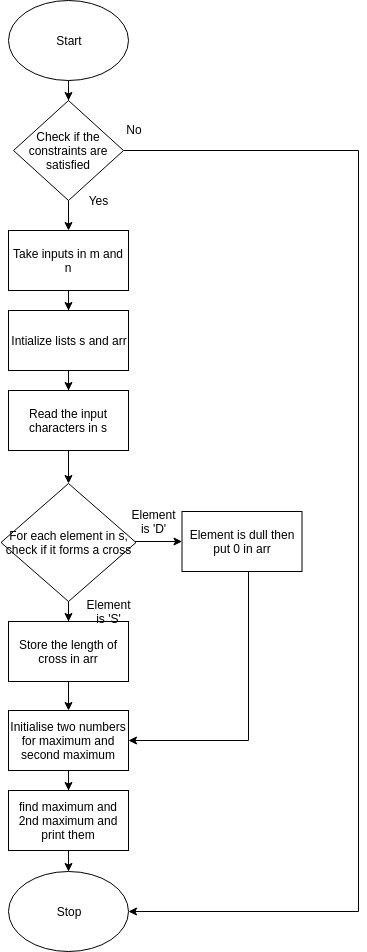
\includegraphics[scale=0.5]{f1.png}
\newpage

\subsection{Screenshots}
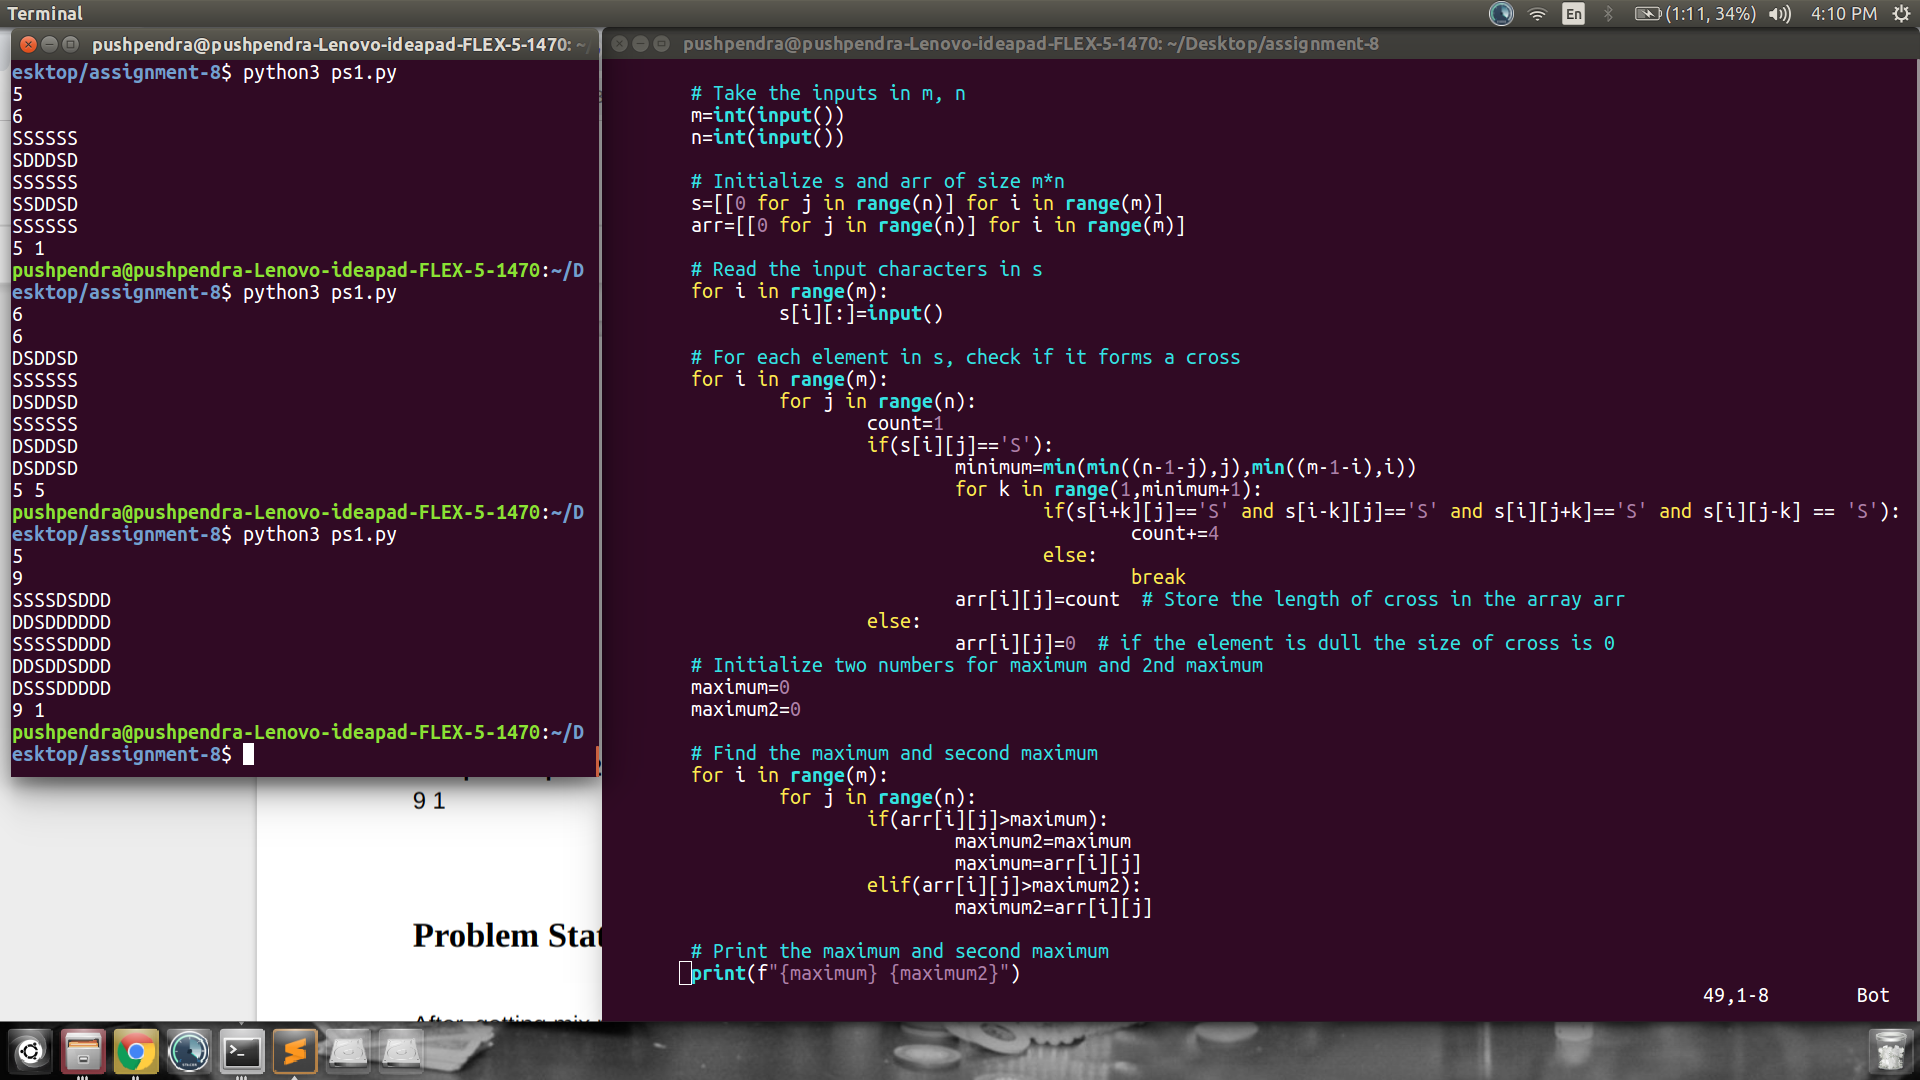
\includegraphics[scale=0.25]{ss1}
\\ \\
\subsection{Difficulties /Issues faced}
NONE
\\
\pagebreak
\section{Problem Statement 2}

{
	\subsection{Problem Statement}{
	After, getting mix results of valid crosses, professors decided to test the computation abilities on one more problem. This time professors wanted to test the decryption capabilities of the computer.\\
	Encryption of  a message requires three keys, k1, k2, and k3. The 26 letters of English and underscore are divided in three groups,  [a-i] form one group, [j-r] a second group, and everything else ([s-z] and underscore) the third group. Within each group the letters are rotated left by ki positions in the message. Each group is rotated independently of the other two. Decrypting the message means doing a right rotation by ki positions within each group.
	\cite{ref2}
	}	
	
	\subsection{Assumptions}
	{
		Input is provided from stdin.
	}
	
	\subsection{Algorithm}
	{
		\begin{enumerate}
			\item Take the inputs in k1, k2, k3 and s
			\item Initailize 3 empty list for the 3 range of characters
			\item Initialize list for output string
			\item Check the character belong to which range
			\item Rotate the elements of list by the value given in k
			\item Place the rotated elements in the out list
			\item Print the out list by converting it to a string
			\item Exit
		\end{enumerate} 
	}
	
	
	\subsection{Input and Output Format}
	{
		\begin{itemize}
			\item 
			
			\textbf{Input format} \\
			All input strings comprises of only lowercase English alphabets and underscores$(\_)$.
			
			Constraints
			\begin{enumerate}
				\item 1 $<=$ Length of the string $<=$150
				\item 1 $<=$ ki $<=$150 (i=1,2,3)
			\end{enumerate}
			\item
			\textbf{Output format} \\
			For each encrypted message, the output is a single line containing the decrypted string.
		\end{itemize}
	}
	
	\subsection{Test Cases}
	\textbf{Input} \\
	2 3 4\\
	dikhtkor$\_$ey$\_$tec$\_$ocsusrsw$\_$ehas$\_$\\	
	\\ \\
	\textbf{Output}\\
	hardwork$\_$is$\_$the$\_$key$\_$to$\_$success\\
	
	\subsection{Flowchart}
	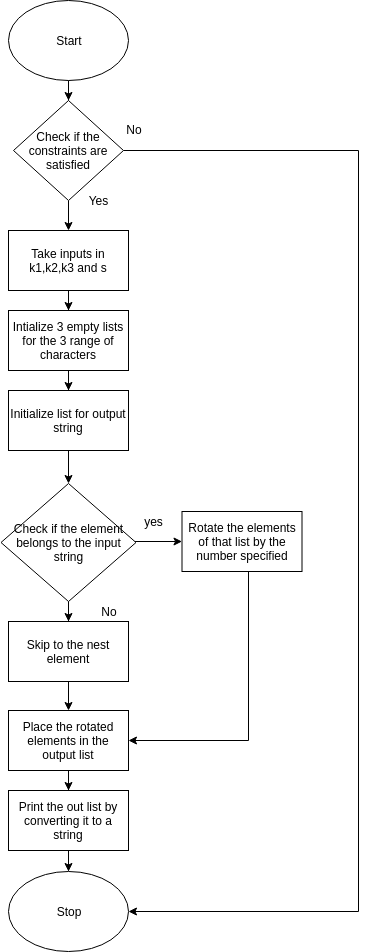
\includegraphics[scale=0.5]{f2.png}
	
	
	\subsection{Screenshots}
	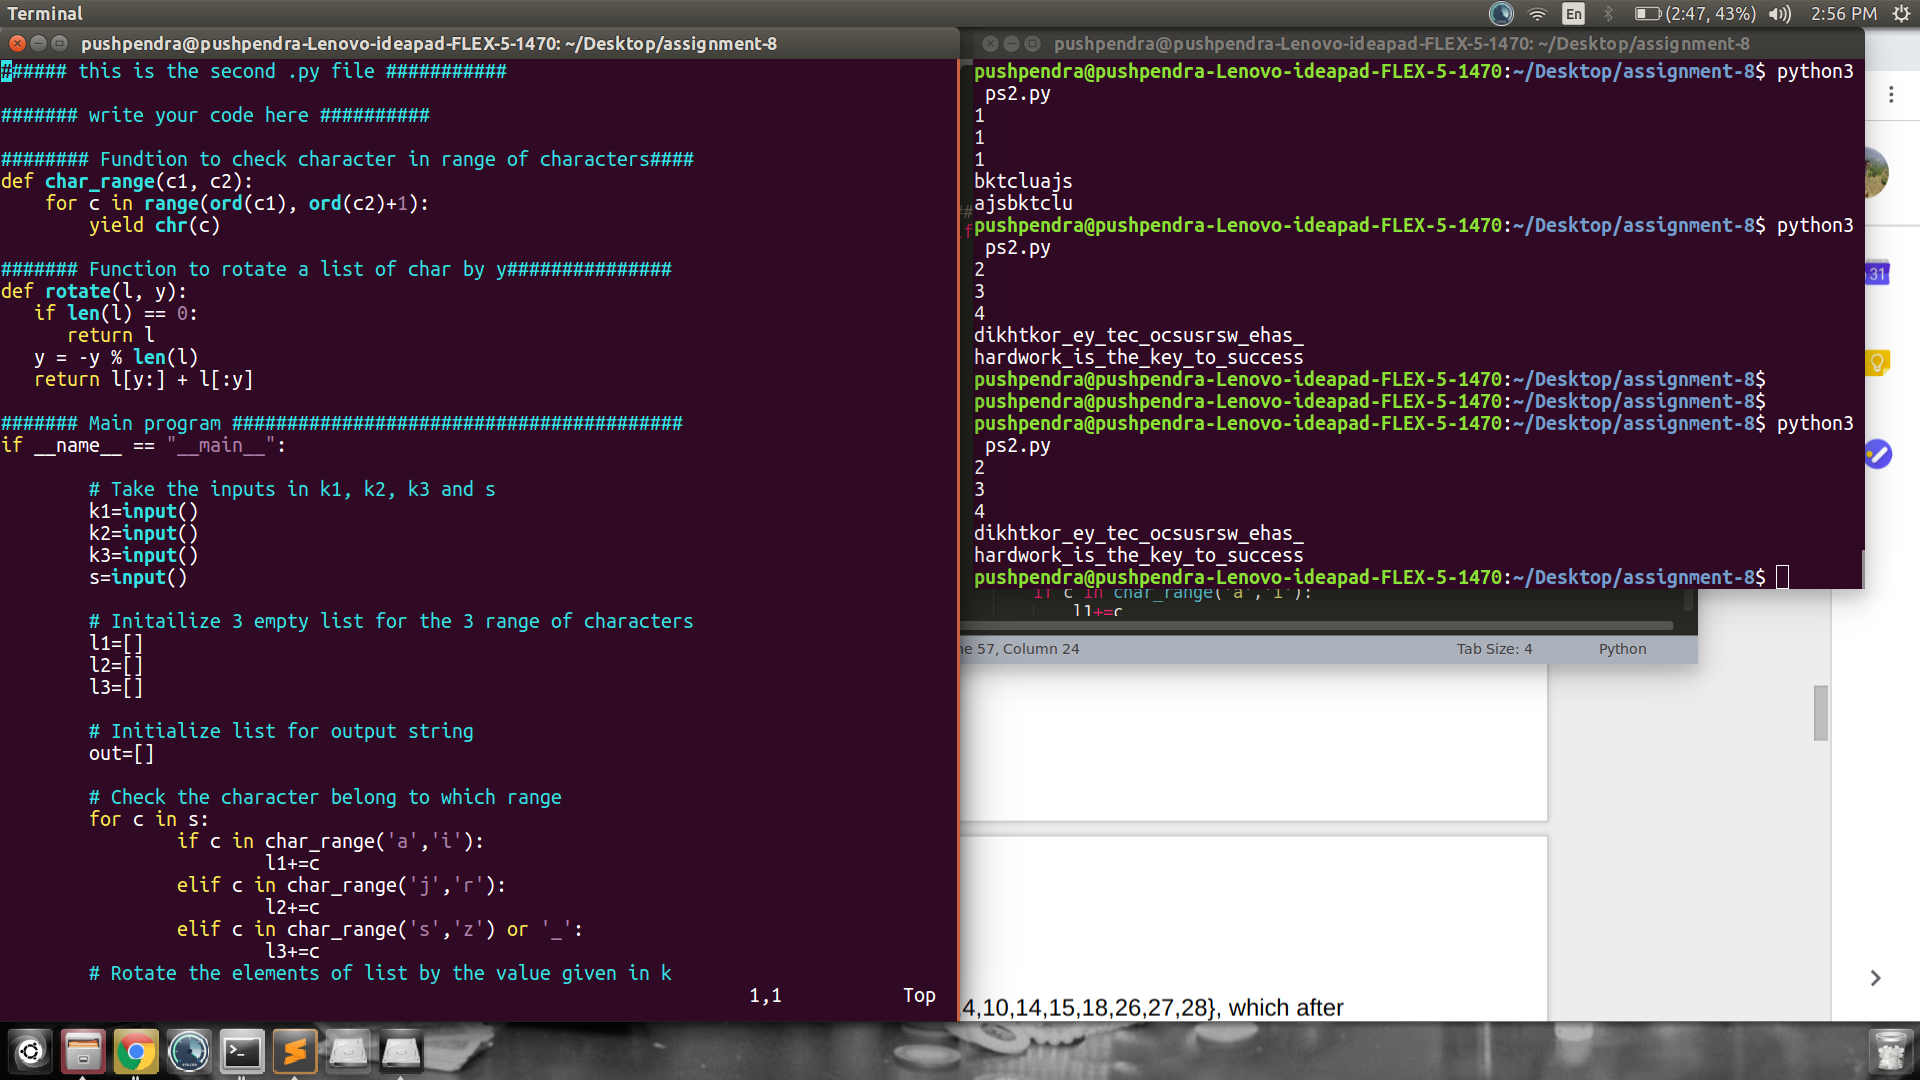
\includegraphics[scale=0.25]{ss2}

	\subsection{Difficulties /Issues faced}
	To join the list back to string
\pagebreak

	\newpage
	\section{Appendix}
	\subsection{Appendix-A: code for ps1}
	\lstinputlisting[language=python, frame = 'single']{ps1.py}  
	\newpage
	\subsection{Appendix-B: code for ps2.l}
	\lstinputlisting[language=python, frame = 'single']{ps2.py}
	\newpage
	\addcontentsline{toc}{section}{References}
	\bibliographystyle{plain}
	\bibliography{document}
\end{document}